Having all optimization statistics continuously aggregated in a repository 
in a common format with JSON meta description 
makes it relatively straightforward to apply various machine learning 
and predictive analytics techniques including 
decision trees, nearest neighbor classifiers, support vector machines (SVM)
and deep learning~\cite{citeulike:873540,sammutencyclopedia}.
%
These techniques can help automate detection of regularities and consistent patterns in program behavior,
build models, and predict efficient optimizations rather than
continuously re-optimizing each new program as we previously demonstrated 
in the MILEPOST project~\cite{29db2248aba45e59:a31e374796869125,CFAP2007}.
%
Furthermore, we can now teach students how to collaboratively model 
the behavior of all computer systems, speed up optimization space exploration, 
and improve predictions of the most efficient software and hardware optimizations
based on various program, data set, platform and run-time 
features~\cite{fursin:hal-01054763,cm:29db2248aba45e59:cd11e3a188574d80}.

   % === CK crowdmodeling ==================================================================
   %CK={"action":"prepare_for_latex", "cid":"slide:5b7be9b27777d3f3", "file":"c5d0a4d5514e4c98-cropped.pdf", "path":"ck-assets", "ck_image":"yes", "ck_image_width":800}
   \begin{figure*}[!htbp]
     \centering
      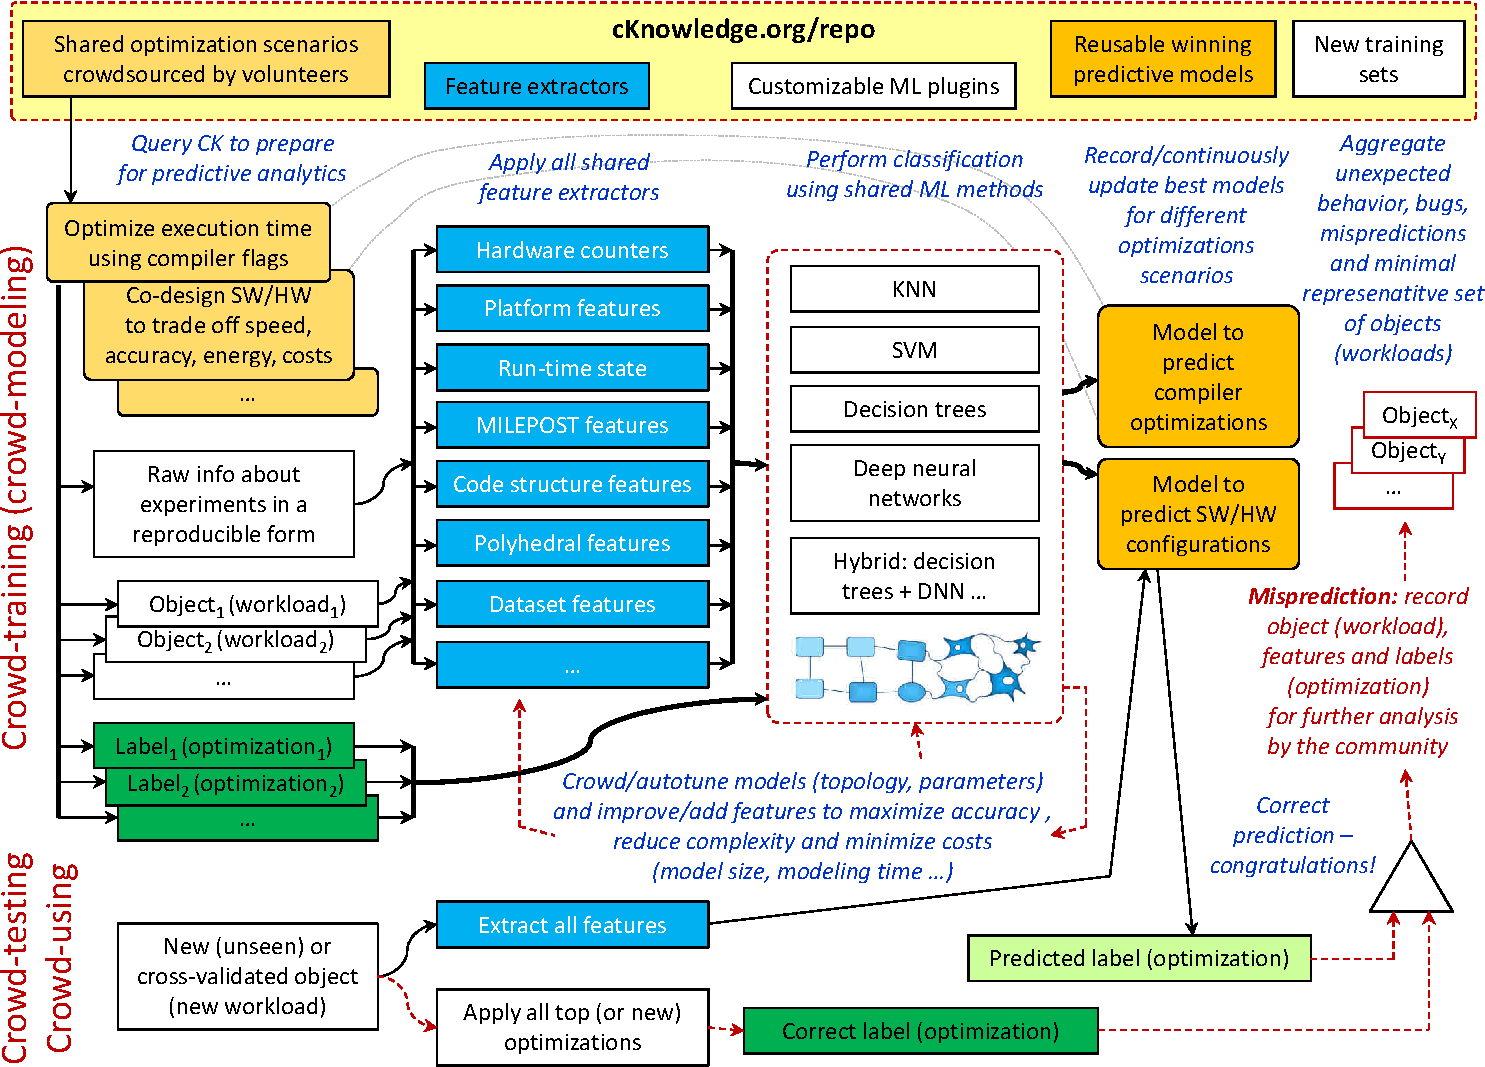
\includegraphics[width=6.6in]
      {ck-assets/c5d0a4d5514e4c98-cropped.pdf} %CK_URL={c5d0a4d5514e4c98-cropped.pdf}
     \caption{
       Universal and high-level Collective Knowledge workflow to connect various communities 
       for collaborative, continuous and semi-automatic learning of multi-objective optimizations
       using shared machine learning modules (plugins) with the unified CK API.
     }
     \label{fig:ck-crowdmodeling}
   \end{figure*}

  % === all model results ==================================================================
  %CK={"action":"prepare_for_latex", "cid":"slide:a0464dc299d2c8dc", "file":"08ac094d04acd157-table.tex", "uid":"f874ed489aa9f313", "path":"ck-assets"}
  %CK={"action":"prepare_for_latex", "cid":"slide:a0464dc299d2c8dc", "file":"08ac094d04acd157-table.html", "uid":"f874ed489aa9f313", "path":"ck-assets"}
  \begin{table*}[!htbp]
    \centering
        \begin{tabular}{|l|p{1.2in}|p{0.9in}|p{0.9in}|}
     \hline
      \textbf{Model} & \textbf{Features} & \textbf{Accuracy (GCC 4.9.2)} & \textbf{Accuracy (GCC 7.1.0)} \\ 
     \hline
      \textbf{ milepost nn } &  ft1 .. ft56  &  0.37  &  0.30 \\
     \hline
    \end{tabular}     %CK_HTML={ck-assets/08ac094d04acd157-table.html}
    \caption{
     Accuracy of the nearest neighbor classifier with MILEPOST features 
     to predict the most efficient combinations of compiler flags 
     for GCC 4.9.2 and GCC 7.1.0 flags on RPi3 device.
    }
    \label{fig:crowdmodeling-milepost-all-rpi3-progs}
  \end{table*}

To demonstrate our approach, we converted all our past research artifacts 
on machine learning based optimization and SW/HW co-design
to CK modules.
%
We then assembled them to a universal Collective Knowledge workflow 
shown in Figure~\ref{fig:ck-crowdmodeling}.
%
If you do not know about machine learning based compiler optimizations, 
we suggest you to start from our MILEPOST GCC paper~\cite{29db2248aba45e59:a31e374796869125}
to make yourself familiar with terminology 
and methodology for machine learning training 
and prediction used further.
%
Next, we will briefly demonstrate the use of this customizable workflow 
to continuously classify shared workloads presented in this report 
in terms of the most efficient compiler optimizations
while using MILEPOST models and features.

   % === CK reactions GCC 4 ==================================================================
   %CK={"action":"prepare_for_latex", "cid":"slide:a0464dc299d2c8dc", "file":"ba5ecb7074b4985a-cropped.pdf", "path":"ck-assets", "ck_image":"yes", "ck_image_width":900}
   %CK={"action":"prepare_for_latex", "cid":"slide:a0464dc299d2c8dc", "file":"8cb40f9e0ee52bcd-cropped.pdf", "path":"ck-assets", "ck_image":"yes", "ck_image_width":900}
   \begin{figure*}[!htbp]
     \centering
      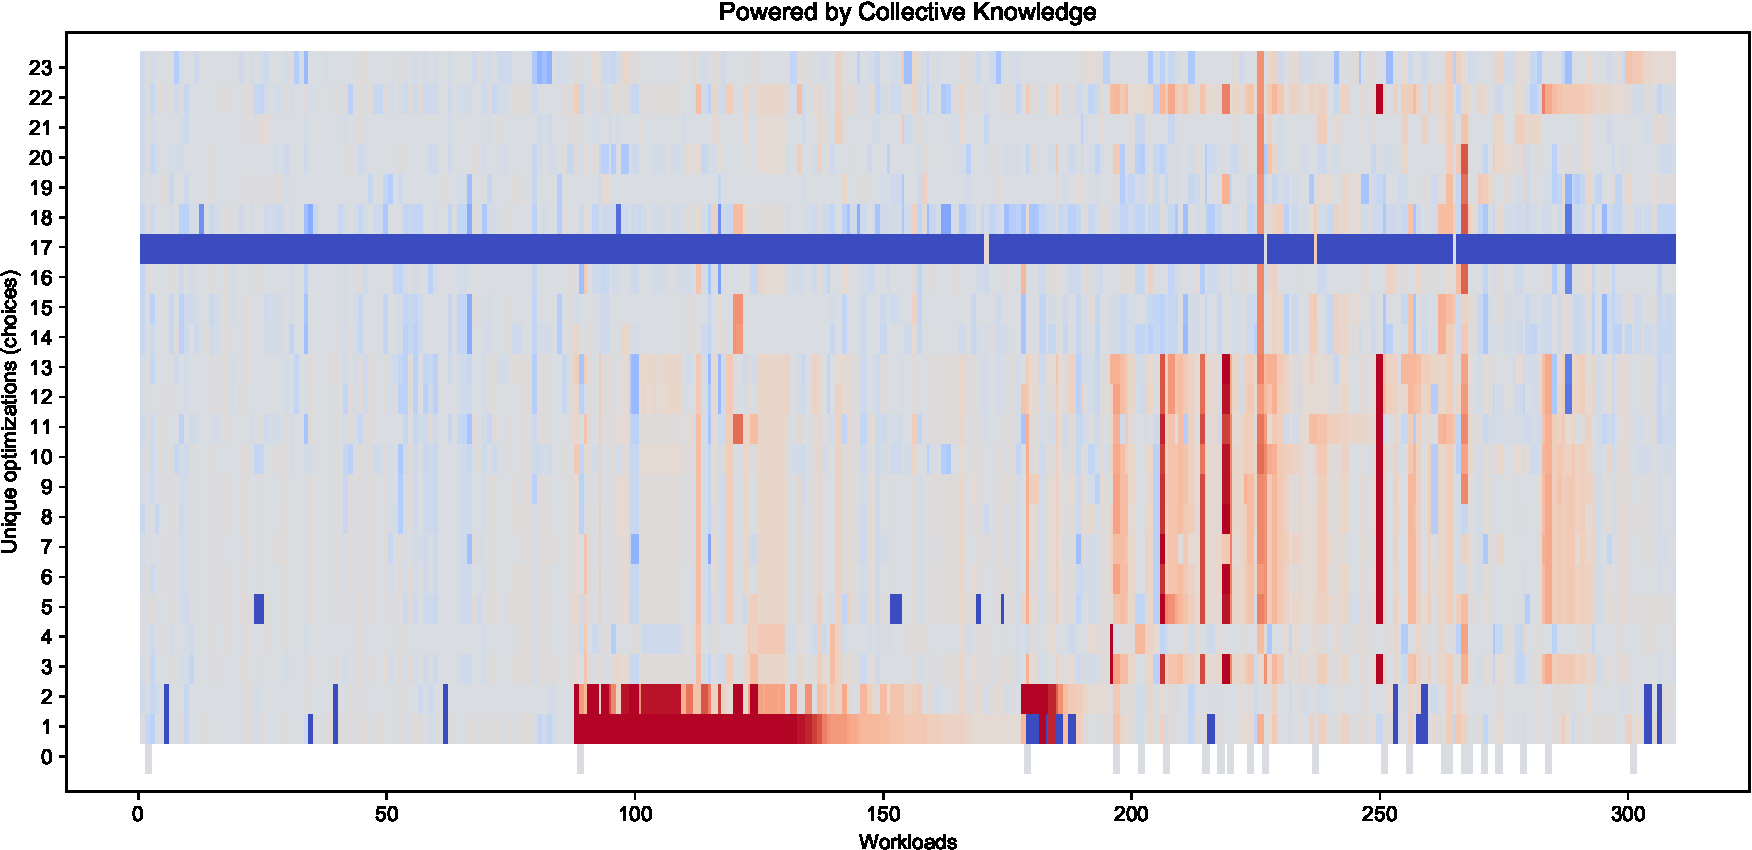
\includegraphics[width=6.6in]
      {ck-assets/ba5ecb7074b4985a-cropped.pdf} %CK_URL={ba5ecb7074b4985a-cropped.pdf}
      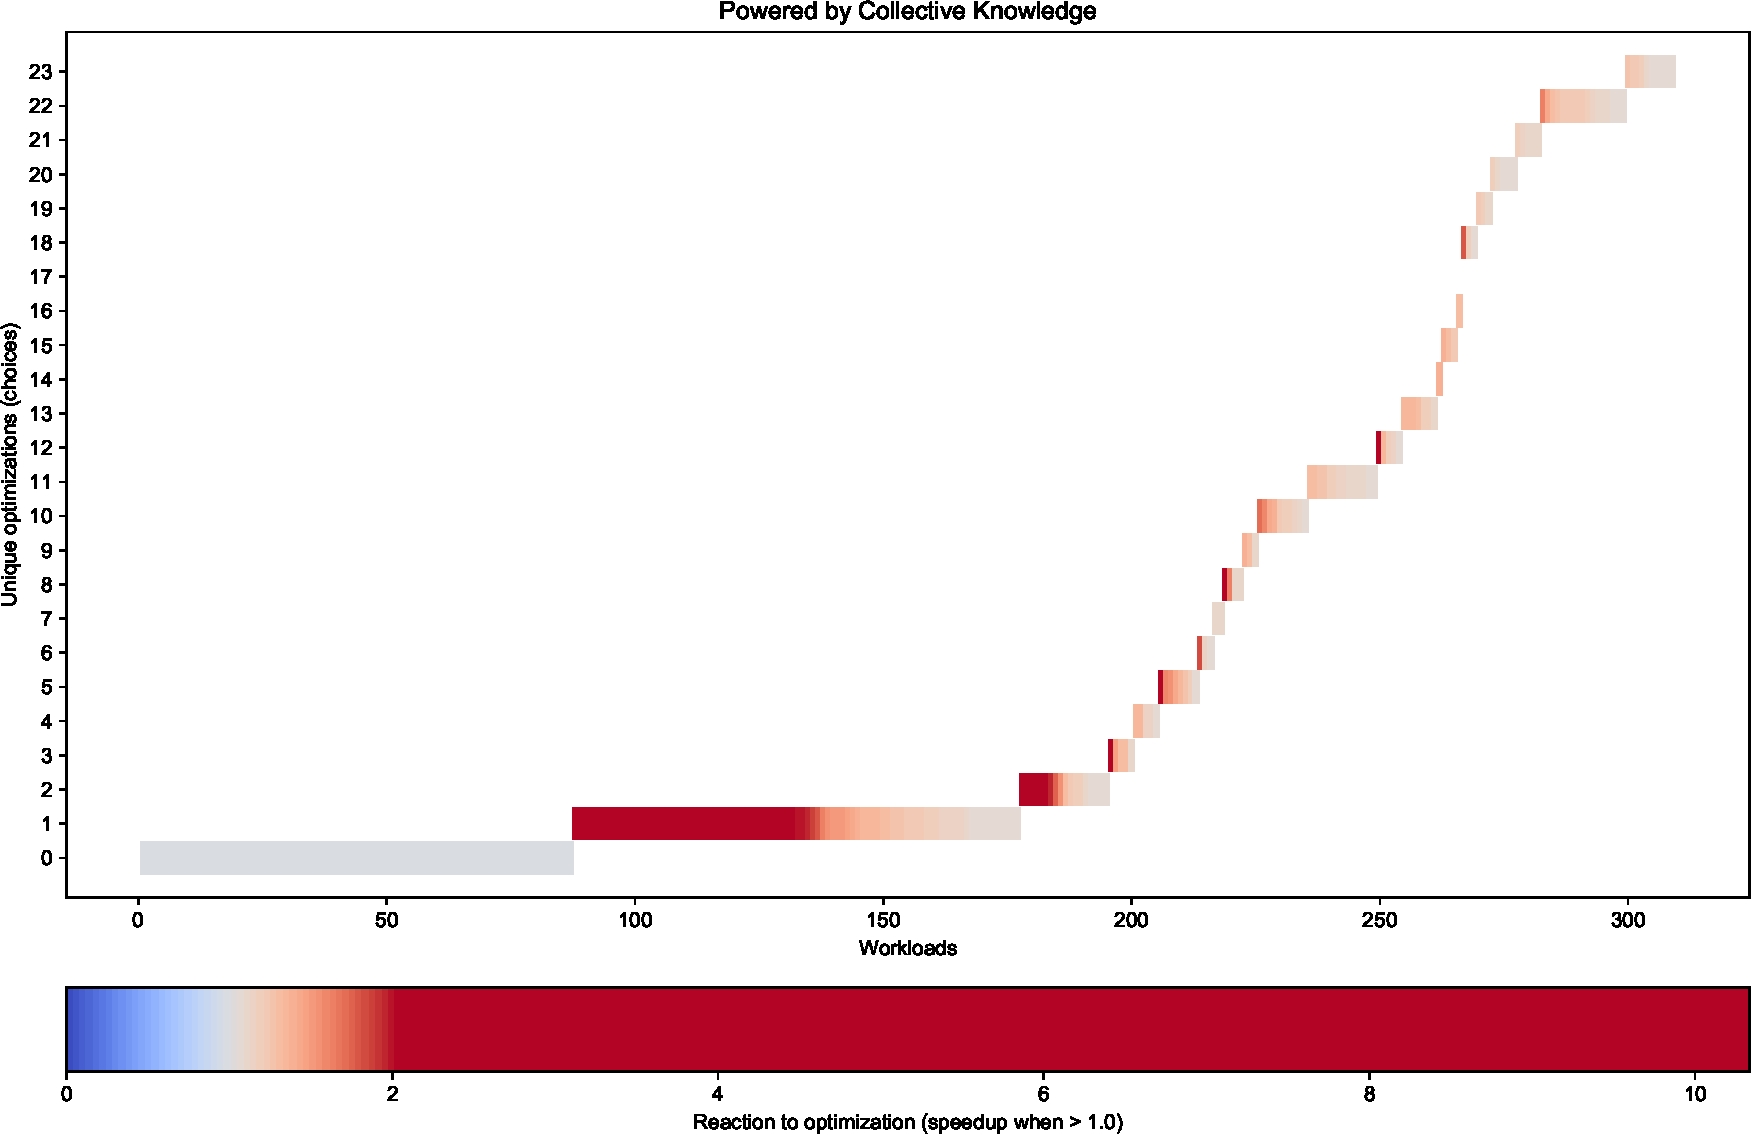
\includegraphics[width=6.6in]
      {ck-assets/8cb40f9e0ee52bcd-cropped.pdf} %CK_URL={8cb40f9e0ee52bcd-cropped.pdf}
     \caption{
       Top graph: reactions of all workloads 
          to all top performing combinations of optimizations
          for GCC 4.9.2 on RPi3 device (speedups if value is more than 1.0).
       Bottom graph: groups of workloads achieving the highest speedup
          for a given unique combination of optimizations.
     }
     \label{fig:ck-reactions-gcc4}
   \end{figure*}

   % === CK reactions GCC 7 ==================================================================
   %CK={"action":"prepare_for_latex", "cid":"slide:a0464dc299d2c8dc", "file":"29119378e09b4dc8-cropped.pdf", "path":"ck-assets", "ck_image":"yes", "ck_image_width":900}
   %CK={"action":"prepare_for_latex", "cid":"slide:a0464dc299d2c8dc", "file":"2d416955df7546b1-cropped.pdf", "path":"ck-assets", "ck_image":"yes", "ck_image_width":900}
   \begin{figure*}[!htbp]
     \centering
      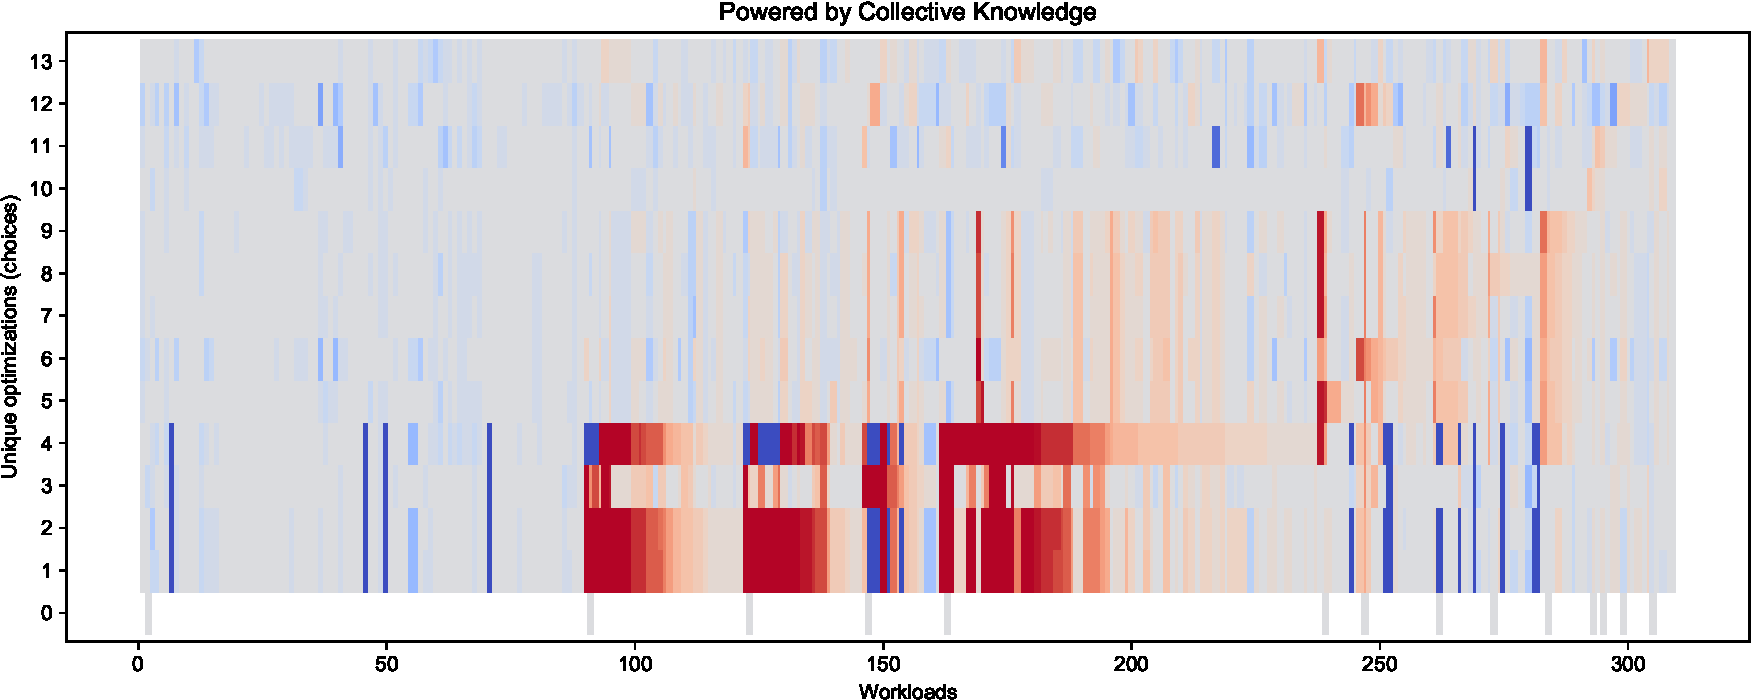
\includegraphics[width=6.6in]
      {ck-assets/29119378e09b4dc8-cropped.pdf} %CK_URL={29119378e09b4dc8-cropped.pdf}
      \vspace{0.1in}
      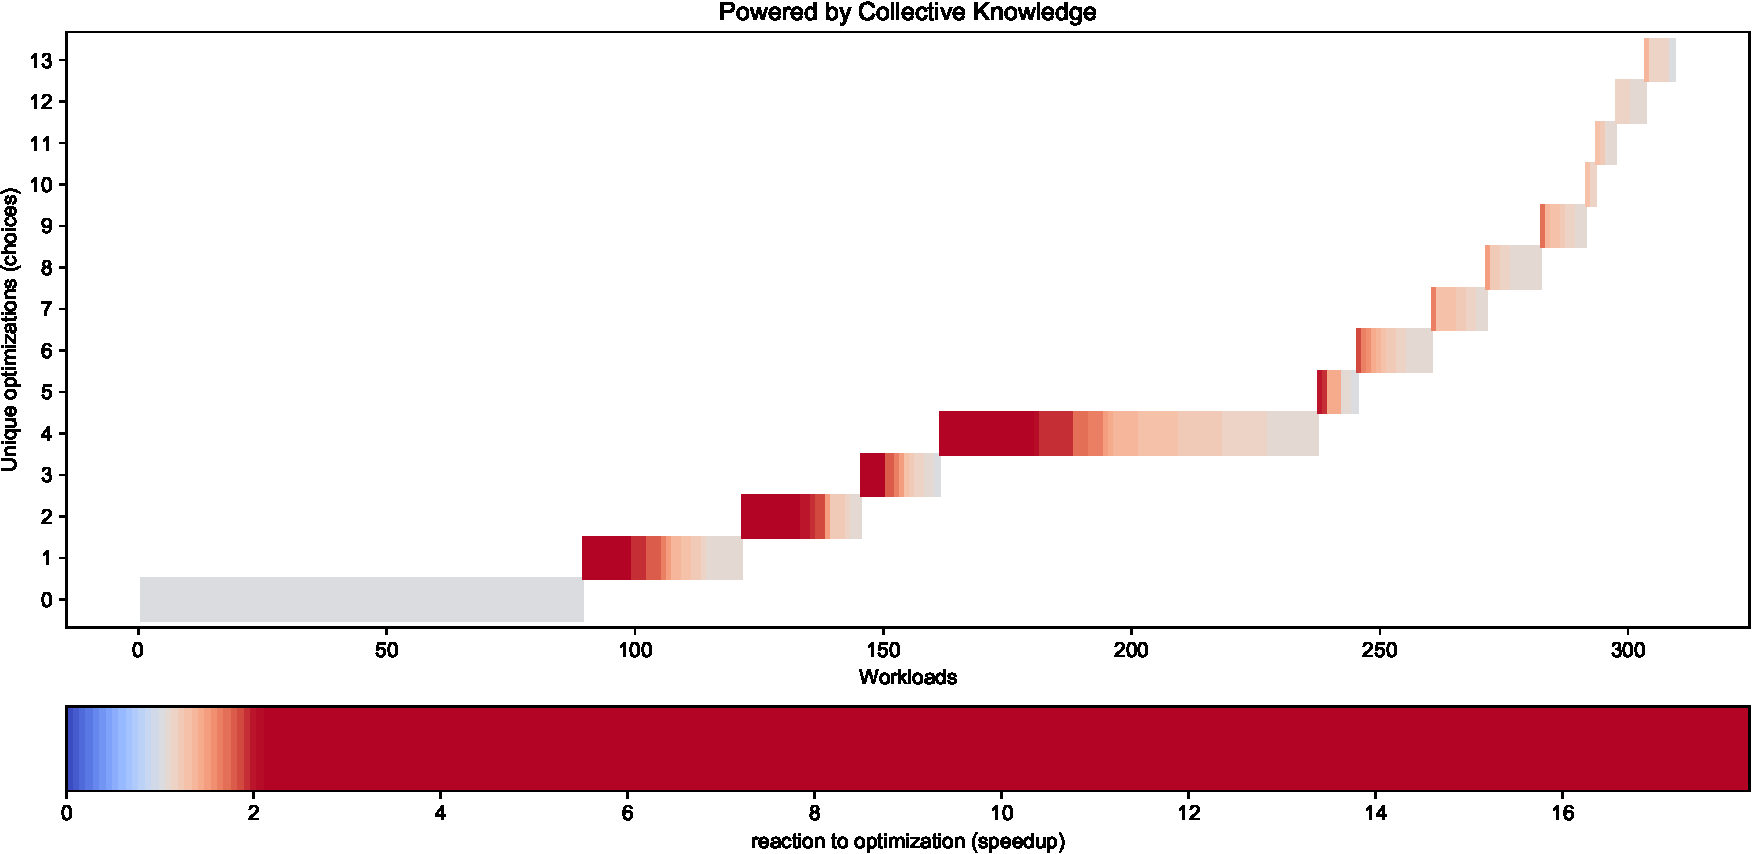
\includegraphics[width=6.6in]
      {ck-assets/2d416955df7546b1-cropped.pdf} %CK_URL={2d416955df7546b1-cropped.pdf}
     \caption{
       Top graph: reactions of all workloads 
          to all top performing combinations of optimizations
          for GCC 7.1.0 on RPi3 device (speedup if value is more than 1.0).
       Bottom graph: groups of workloads achieving the highest speedup
          for a given unique combination of optimizations.
     }
     \label{fig:ck-reactions-gcc7}
   \end{figure*}

First, we query the public CK repository~\cite{live-ck-repo}
to collect all optimization statistics together with all associated objects 
(workloads, data sets, platforms) for a given optimization scenario. 
%
In our compiler flag optimization scenario, we retrieve all
most efficient compiler flags combinations found and shared
by the community when crowd-tuning GCC 4.9.2 on RPi3 device
(Figure~\ref{fig:ck-snapshot-of-results-gcc4}).

Note that our CK crowd-tuning workflow also continuously apply
such optimization to all shared workloads.
%
This allows us to analyze "reaction" of any given workload 
to all most efficient optimizations.
%
We can then group together those workloads which exhibit similar reactions.

The top graph in Figure~\ref{fig:ck-reactions-gcc4} shows reactions of all workloads 
to the most efficient optimizations as a ratio of the default execution time (-O3) 
to the execution time of applied optimization.
%
It confirms yet again (\cite{cm:29db2248aba45e59:cd11e3a188574d80}) that there is no single "winning" 
combination of optimizations and they can either considerably improve or degrade execution time 
on different workloads.
%
It also confirms that it is indeed possible to group together multiple workloads 
which share the most efficient combination of compiler flags, i.e. which achieve 
the highest speedup for a common optimization as shown in the bottom graph 
in Figure~\ref{fig:ck-reactions-gcc4}.
%
Figure~\ref{fig:ck-reactions-gcc7} shows similar trends for GCC 7.1.0 on the same RPi3 device
even though the overall number of the most efficient combinations of compiler flags is smaller 
than for GCC 4.9.2 likely due to considerably improved internal optimization heuristics over past years
(see Figure~\ref{fig:ck-snapshot-of-results-gcc7}).

Having such groups of labeled objects (where labels are the most efficient optimizations
and objects are workloads) allows us to use standard machine learning classification methodology.
%
One must find such a set of objects' features and a model which maximizes 
correct labeling of previously unseen objects, or in our cases can correctly predict 
the most efficient software optimization and hardware design for a given workload.
%
As example, we extracted 56 so-called MILEPOST features described in~\cite{29db2248aba45e59:a31e374796869125} 
(static program properties extracted from GCC's intermediate representation) 
from all shared programs, stored them in \emph{program.static.features},
and applied simple nearest neighbor classifier to above data.
%
We then evaluated the quality of such model (ability to predict) using prediction accuracy
during standard leave-one-out cross-validation technique: for each workload we remove it
from the training set, build a model, validate predictions, sum up all correct predictions 
and divide by the total number of workloads.

Table~\ref{fig:crowdmodeling-milepost-all-rpi3-progs} shows this prediction accuracy
of our MILEPOST model for compiler flags from GCC 4.9.2 and GCC 7.1.0 
across all shared workloads on RPi3 device.
%
One may notice that it is nearly twice lower than in the
original MILEPOST
paper~\cite{29db2248aba45e59:a31e374796869125}.
%
As we explain in~\cite{cm:29db2248aba45e59:cd11e3a188574d80},
in the MILEPOST project we could only use a dozen of similar
workloads and just a few most efficient optimizations to be
able to perform all necessary experiments within a reasonable
amount of time (6 months).
%
After brining the community on hoard, we could now use a much larger 
collective training set with more than 300 shared, diverse 
and non-synthesized workloads while analyzing much more optimizations 
by crowdsourcing autotuning.
%
This helps obtain a more realistic limit of the MILEPOST predictor.

Though relatively low, this number can now become a 
reference point to be further improved by the community.
%
It is similar in spirit to the ImageNet Large Scale Visual Recognition Competition
(ILSVRC)~\cite{DBLP:journals/corr/RussakovskyDSKSMHKKBBF14}
which reduced image classification error rate from 25\%
in 2011 to just a few percent with the help of the community.
%
Furthermore, we can also keep just a few representative
workloads for each representative group as well as misclassified ones in
a public repository thus producing a minimized, realistic and
representative training set for systems researchers.

\textit{We shared all demo scripts which we used to generate data and
graphs in this section in the following CK entry (however they are not yet
user-friendly and we will continue improving documentation and
standardizing APIs of reusable CK modules with the help of the community):}

\begin{flushleft}
\texttt{\$ ck find script:rpi3-crowdmodel}
\end{flushleft}
